%
% This is the LaTeX template file for lecture notes for EE 382C/EE 361C.
%
% To familiarize yourself with this template, the body contains
% some examples of its use.  Look them over.  Then you can
% run LaTeX on this file.  After you have LaTeXed this file then
% you can look over the result either by printing it out with
% dvips or using xdvi.
%
% This template is based on the template for Prof. Sinclair's CS 270.

\documentclass[twoside]{article}
\usepackage{graphics}
\usepackage{graphicx}
\usepackage{float}
\setlength{\oddsidemargin}{0.25 in}
\setlength{\evensidemargin}{-0.25 in}
\setlength{\topmargin}{-0.6 in}
\setlength{\textwidth}{6.5 in}
\setlength{\textheight}{8.5 in}
\setlength{\headsep}{0.75 in}
\setlength{\parindent}{0 in}
\setlength{\parskip}{0.1 in}

%
% The following commands set up the lecnum (lecture number)
% counter and make various numbering schemes work relative
% to the lecture number.
%
\newcounter{lecnum}
\renewcommand{\thepage}{\thelecnum-\arabic{page}}
\renewcommand{\thesection}{\thelecnum.\arabic{section}}
\renewcommand{\theequation}{\thelecnum.\arabic{equation}}
\renewcommand{\thefigure}{\thelecnum.\arabic{figure}}
\renewcommand{\thetable}{\thelecnum.\arabic{table}}

%
% The following macro is used to generate the header.
%
\newcommand{\lecture}[4]{
   \pagestyle{myheadings}
   \thispagestyle{plain}
   \newpage
   \setcounter{lecnum}{#1}
   \setcounter{page}{1}
   \noindent
   \begin{center}
   \framebox{
      \vbox{\vspace{2mm}
    \hbox to 6.28in { {\bf EE 382C/361C: Multicore Computing
                        \hfill Fall 2016} }
       \vspace{4mm}
       \hbox to 6.28in { {\Large \hfill Lecture #1: #2  \hfill} }
       \vspace{2mm}
       \hbox to 6.28in { {\it Lecturer: #3 \hfill Scribe: #4} }
      \vspace{2mm}}
   }
   \end{center}
   \markboth{Lecture #1: #2}{Lecture #1: #2}
   %{\bf Disclaimer}: {\it These notes have not been subjected to the
   %usual scrutiny reserved for formal publications.  They may be distributed
   %outside this class only with the permission of the Instructor.}
   \vspace*{4mm}
}

%
% Convention for citations is authors' initials followed by the year.
% For example, to cite a paper by Leighton and Maggs you would type
% \cite{LM89}, and to cite a paper by Strassen you would type \cite{S69}.
% (To avoid bibliography problems, for now we redefine the \cite command.)
% Also commands that create a suitable format for the reference list.
\renewcommand{\cite}[1]{[#1]}
\def\beginrefs{\begin{list}%
        {[\arabic{equation}]}{\usecounter{equation}
         \setlength{\leftmargin}{2.0truecm}\setlength{\labelsep}{0.4truecm}%
         \setlength{\labelwidth}{1.6truecm}}}
\def\endrefs{\end{list}}
\def\bibentry#1{\item[\hbox{[#1]}]}

%Use this command for a figure; it puts a figure in wherever you want it.
%usage: \fig{NUMBER}{SPACE-IN-INCHES}{CAPTION}
\newcommand{\fig}[3]{
			\vspace{#2}
			\begin{center}
			Figure \thelecnum.#1:~#3
			\end{center}
	}
% Use these for theorems, lemmas, proofs, etc.
\newtheorem{theorem}{Theorem}[lecnum]
\newtheorem{lemma}[theorem]{Lemma}
\newtheorem{proposition}[theorem]{Proposition}
\newtheorem{claim}[theorem]{Claim}
\newtheorem{corollary}[theorem]{Corollary}
\newtheorem{definition}[theorem]{Definition}
\newenvironment{proof}{{\bf Proof:}}{\hfill\rule{2mm}{2mm}}

% **** IF YOU WANT TO DEFINE ADDITIONAL MACROS FOR YOURSELF, PUT THEM HERE:

\begin{document}
%FILL IN THE RIGHT INFO.
%\lecture{**LECTURE-NUMBER**}{**DATE**}{**LECTURER**}{**SCRIBE**}
\lecture{10}{September 27}{Vijay Garg}{Prateek Srivastava}
%\footnotetext{These notes are partially based on those of Nigel Mansell.}

% **** YOUR NOTES GO HERE:

% Some general latex examples and examples making use of the
% macros follow.  
%**** IN GENERAL, BE BRIEF. LONG SCRIBE NOTES, NO MATTER HOW WELL WRITTEN,
%**** ARE NEVER READ BY ANYBODY.
\section{Introduction}
This lecture covers following items.
\begin{itemize}
\item Project outlines
\item Merging Puzzle
\item Consistency conditions
\end{itemize}


\section{Projects}

Projects need to be done in groups of 2 or 3. Undergrads should do project with other undergrads while grads with grads. For undergrads, aim would be to implement and turn in just one plot of the observations. For grads, they need to pick a topic, implement it and possibly improve on it. Topics can be chosen from recent conference proceedings as well.\\
If undergrads choose same topics, they can compete among themselves for the performance. 
Topics are posted on canvas. A brief overview is present here.\\
\begin{itemize}
\item Mutex algorithms not covered in class can be implemented e.g. colored bakery.
\item Monitors with additional feature like abort.
\item Parallel work scheduling and work distribution algorithms using some language e.g. language CILK.
\item Concurrent trees, queues and skiplist. Avoids serialization by locking.
\item Concurrent Hash-tables like Cuckoo Hashing, and Hopscotch Hashing.
\item Poset, lattice theory. some part will be covered in class.
\item Graph shortest path, spanning trees, max flows can be implemented on stampede on GPU.
\item Implement sorting and compare performance.
\item Image processing on GPU, scientific computation like fft and polynomial. Data mining algorithms like K-means.
\item Text analysis used heavily by Google, pattern matching.
\item Iphone/Android for this topic need to give exact details on what the app is going to do.
\item Run model checker on algorithm and verify correctness.
\item Lamport's Temporal Logic of Actions for specifying and verifying the correctness of concurrent algorithms.
\item Verification of consistency conditions.
\end{itemize}
The project should contain some references.  

\section{Merge Puzzle contd\ldots}
\subsection{Problem}
Merge two sorted arrays of length n to form a sorted array of length 2n.

\subsection{Solutions}
(a) Sequential algorithm was like the merge sort.\\
(b) Parallel algorithm computes rank for each element which is the index into the final merged array. Each element computes its rank, using its own position and its position in the other array using binary search.\\
Following table summarizes the time and work complexity of already discussed solution.
\begin{table}[h]
\centering
\label{my-label}
\begin{tabular}{|l|l|l|}
\hline
           & Time     & Work       \\ \hline
Sequential & O(n)     & O(n)       \\ \hline
Parallel   & O(log n) & O(n log n) \\ \hline
\end{tabular}
\end{table}
\subsection{Work optimal parallel solution}
We would like to reduce the work from \(O(n*logn)\). This can be achieved using cascaded algorithm.\\ Divide the input array in log n groups. The starting element in each group is called the splitter.\\
No. of splitters = \( O\left(\frac{n}{log n}\right)\)\\
\begin{figure}[H]
  \centering
  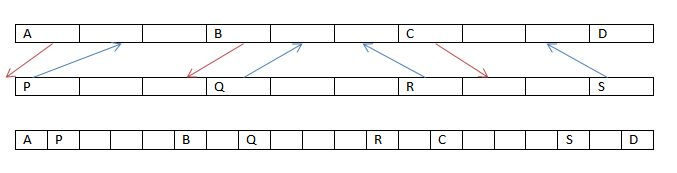
\includegraphics[height=0.250\textheight, width=0.750\linewidth]{1.PNG} 
  \caption{Merging Sorted Arrays}
  \label{fig:1}
\end{figure}
Fill the splitter in the target array by finding ranks as done in the parallel algorithm as shown in the figure\\
Find the sublist in first list say, $\alpha$ and second list say, $\beta$ such that they are in between the splitters.\\
Number of such lists = \( O\left(\frac{n}{log n}\right)\)\\
Size of each list = \(Olog n)\)\\
We know that the \(log n\) size lists can be merged in \(Olog n)\) using the sequential algorithm.\\ 

Following table summarizes the steps.
\begin{table}[h]
\centering
\label{my-label1}
\begin{tabular}{|l|l|l|}
\hline
       & Time     & Work \\ \hline
Step 1 & O(log n) & O(n) \\ \hline
Step 2 & O(log n) & O(n) \\ \hline
Total  & O(log n) & O(n) \\ \hline
\end{tabular}
\end{table}
Hence, the solution is work as well as time optimal. Although, there are solutions optimal then this one as well.
\section{Parallel prefix sum puzzle}
Given an array find an output array such that each element in output array is sum of input array elements till that index.\\
e.g. Input   3, 4, 19, 11, 13\\
$\-$  $\-$ $\-$ $\-$ Output  3, 7, 26, 37, 50\\
The algorithm is called scan.
\section{Consistency condition}
Consider a stack with following operations\\
$\-$  $\-$ $\-$ $\-$push(40) push(9) pop (Pop should return 9 not 40)\\This is sequential correctness\\
Now consider following situation.\\
\begin{figure}[H]
  \centering
  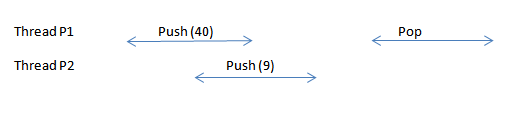
\includegraphics[height=0.2\textheight, width=0.6\linewidth]{2.PNG} 
  \label{fig:2}
\end{figure}
The correctness of output depends on the definition of correct output. Lamport wrote a 2 page paper explaining what it means to be sequentially consistent in a multiprocessor environment.

\subsection{Notations}
A method call is split into two events
\begin{list}{*}{•}
\item {\em Invocation} method name + args e.g. f.foo(arg1, arg2)
\item {\em Response} result or exception
\end{list}

Consider, P f.foo(arg1, arg2)\\
This is an invocation of object f on thread P\\
foo is method name \\
arg1, arg2 are arguments\\
Consider, P f.response \\
This is the return value, for object f on thread P\\

We define following\\
$\-$  $\-$ $\-$ inv(e) is invocation of e\\
$\-$  $\-$ $\-$ resp(e) is response of e\\
$\-$  $\-$ $\-$ proc(e) is process on which e runs\\
\subsection{History}
A sequence of invocations and responses constitutes history.\\	
History  $(H, <_H)$ is set of operations in real time order.\\
The relation $e <_H f$ holds, if resp(e) occurred before inv(f)\\
\begin{figure}[H]
  \centering
  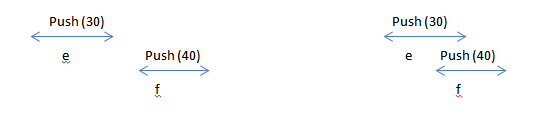
\includegraphics[height=0.20\textheight, width=0.80\linewidth]{3.PNG} 
  \label{fig:3}
\end{figure}
In first case, response of e occurs before invocation of f. In second case, 
e overlaps with f or is concurrent with f. There is no particular order\\

The relation $<_H$ is\\ (a) irreflexive (each element does not satisfy the relation with itself)\\ 
		(b)	transitive (if relation applies between successive members of a sequence, it must also apply between any two members taken in order)\\
This two conditions imply that the relation is asymmetric.\\
Since the relation $(H, <_H)$ is irreflexive and transitive, $(H, <_H)$ is a partial ordered set (poset).\\
\subsection{Process Order}
$e < f$ is in process order if 
\begin{list}{•}{•}
\item proc(e) = proc(f)
\item resp(e) occurred before inv(f)
\end{list}
\subsection{Total order}
A poset $(H, <_H)$ is a total order if for all distinct x,y $(<_X)$, satisfies $(x<y)$ or $(y<x)$\\ 
\subsection{Sequential History}
A history $(H, <_H)$ is sequential if $(<_H)$ is a total order.\\
A sequential history is legal if it satisfies sequential specs of the objects.\\
\section*{References}
\beginrefs
\bibentry{1}{\sc V. K. Garg}, Introduction to Multicore Computing
\endrefs
\end{document}





